\documentclass[twoside]{book}

% Packages required by doxygen
\usepackage{fixltx2e}
\usepackage{calc}
\usepackage{doxygen}
\usepackage[export]{adjustbox} % also loads graphicx
\usepackage{graphicx}
\usepackage[utf8]{inputenc}
\usepackage{makeidx}
\usepackage{multicol}
\usepackage{multirow}
\PassOptionsToPackage{warn}{textcomp}
\usepackage{textcomp}
\usepackage[nointegrals]{wasysym}
\usepackage[table]{xcolor}

% Font selection
\usepackage[T1]{fontenc}
\usepackage[scaled=.90]{helvet}
\usepackage{courier}
\usepackage{amssymb}
\usepackage{sectsty}
\renewcommand{\familydefault}{\sfdefault}
\allsectionsfont{%
  \fontseries{bc}\selectfont%
  \color{darkgray}%
}
\renewcommand{\DoxyLabelFont}{%
  \fontseries{bc}\selectfont%
  \color{darkgray}%
}
\newcommand{\+}{\discretionary{\mbox{\scriptsize$\hookleftarrow$}}{}{}}

% Page & text layout
\usepackage{geometry}
\geometry{%
  a4paper,%
  top=2.5cm,%
  bottom=2.5cm,%
  left=2.5cm,%
  right=2.5cm%
}
\tolerance=750
\hfuzz=15pt
\hbadness=750
\setlength{\emergencystretch}{15pt}
\setlength{\parindent}{0cm}
\setlength{\parskip}{3ex plus 2ex minus 2ex}
\makeatletter
\renewcommand{\paragraph}{%
  \@startsection{paragraph}{4}{0ex}{-1.0ex}{1.0ex}{%
    \normalfont\normalsize\bfseries\SS@parafont%
  }%
}
\renewcommand{\subparagraph}{%
  \@startsection{subparagraph}{5}{0ex}{-1.0ex}{1.0ex}{%
    \normalfont\normalsize\bfseries\SS@subparafont%
  }%
}
\makeatother

% Headers & footers
\usepackage{fancyhdr}
\pagestyle{fancyplain}
\fancyhead[LE]{\fancyplain{}{\bfseries\thepage}}
\fancyhead[CE]{\fancyplain{}{}}
\fancyhead[RE]{\fancyplain{}{\bfseries\leftmark}}
\fancyhead[LO]{\fancyplain{}{\bfseries\rightmark}}
\fancyhead[CO]{\fancyplain{}{}}
\fancyhead[RO]{\fancyplain{}{\bfseries\thepage}}
\fancyfoot[LE]{\fancyplain{}{}}
\fancyfoot[CE]{\fancyplain{}{}}
\fancyfoot[RE]{\fancyplain{}{\bfseries\scriptsize Generated by Doxygen }}
\fancyfoot[LO]{\fancyplain{}{\bfseries\scriptsize Generated by Doxygen }}
\fancyfoot[CO]{\fancyplain{}{}}
\fancyfoot[RO]{\fancyplain{}{}}
\renewcommand{\footrulewidth}{0.4pt}
\renewcommand{\chaptermark}[1]{%
  \markboth{#1}{}%
}
\renewcommand{\sectionmark}[1]{%
  \markright{\thesection\ #1}%
}

% Indices & bibliography
\usepackage{natbib}
\usepackage[titles]{tocloft}
\setcounter{tocdepth}{3}
\setcounter{secnumdepth}{5}
\makeindex

% Hyperlinks (required, but should be loaded last)
\usepackage{ifpdf}
\ifpdf
  \usepackage[pdftex,pagebackref=true]{hyperref}
\else
  \usepackage[ps2pdf,pagebackref=true]{hyperref}
\fi
\hypersetup{%
  colorlinks=true,%
  linkcolor=blue,%
  citecolor=blue,%
  unicode%
}

% Custom commands
\newcommand{\clearemptydoublepage}{%
  \newpage{\pagestyle{empty}\cleardoublepage}%
}

\usepackage{caption}
\captionsetup{labelsep=space,justification=centering,font={bf},singlelinecheck=off,skip=4pt,position=top}

%===== C O N T E N T S =====

\begin{document}

% Titlepage & ToC
\hypersetup{pageanchor=false,
             bookmarksnumbered=true,
             pdfencoding=unicode
            }
\pagenumbering{alph}
\begin{titlepage}
\vspace*{7cm}
\begin{center}%
{\Large Versuch08 }\\
\vspace*{1cm}
{\large Generated by Doxygen 1.8.13}\\
\end{center}
\end{titlepage}
\clearemptydoublepage
\pagenumbering{roman}
\tableofcontents
\clearemptydoublepage
\pagenumbering{arabic}
\hypersetup{pageanchor=true}

%--- Begin generated contents ---
\chapter{Main Page}
\label{index}\hypertarget{index}{}Dokumentation des Spiels Reversi im Rahmen des Praktikums Informatik 1.

\begin{DoxyAuthor}{Author}
Can Oezmaden 
\end{DoxyAuthor}
\begin{DoxyDate}{Date}
2017 
\end{DoxyDate}

\chapter{Hierarchical Index}
\section{Class Hierarchy}
This inheritance list is sorted roughly, but not completely, alphabetically\+:\begin{DoxyCompactList}
\item \contentsline{section}{Expression}{\pageref{class_expression}}{}
\begin{DoxyCompactList}
\item \contentsline{section}{Add}{\pageref{class_add}}{}
\item \contentsline{section}{Const}{\pageref{class_const}}{}
\item \contentsline{section}{Div}{\pageref{class_div}}{}
\item \contentsline{section}{Mul}{\pageref{class_mul}}{}
\item \contentsline{section}{Result}{\pageref{class_result}}{}
\item \contentsline{section}{Sub}{\pageref{class_sub}}{}
\end{DoxyCompactList}
\end{DoxyCompactList}

\chapter{Class Index}
\section{Class List}
Here are the classes, structs, unions and interfaces with brief descriptions\+:\begin{DoxyCompactList}
\item\contentsline{section}{\hyperlink{class_add}{Add} \\*Addition expression }{\pageref{class_add}}{}
\item\contentsline{section}{\hyperlink{class_const}{Const} \\*Saves a value for further calculation }{\pageref{class_const}}{}
\item\contentsline{section}{\hyperlink{class_div}{Div} \\*Division expression }{\pageref{class_div}}{}
\item\contentsline{section}{\hyperlink{class_expression}{Expression} \\*Abstract \hyperlink{class_expression}{Expression} Class }{\pageref{class_expression}}{}
\item\contentsline{section}{\hyperlink{class_mul}{Mul} \\*Multiplication expression }{\pageref{class_mul}}{}
\item\contentsline{section}{\hyperlink{class_result}{Result} \\*Calculates and saves the result }{\pageref{class_result}}{}
\item\contentsline{section}{\hyperlink{class_sub}{Sub} \\*Subtraction expression }{\pageref{class_sub}}{}
\end{DoxyCompactList}

\chapter{File Index}
\section{File List}
Here is a list of all documented files with brief descriptions\+:\begin{DoxyCompactList}
\item\contentsline{section}{\hyperlink{add_8cpp}{add.\+cpp} \\*Contains the method declarations used in the \hyperlink{class_add}{Add} Class }{\pageref{add_8cpp}}{}
\item\contentsline{section}{\hyperlink{add_8h}{add.\+h} \\*Header file for the \hyperlink{class_add}{Add} Class }{\pageref{add_8h}}{}
\item\contentsline{section}{\hyperlink{const_8cpp}{const.\+cpp} \\*Contains the method declarations used in the \hyperlink{class_const}{Const} Class }{\pageref{const_8cpp}}{}
\item\contentsline{section}{\hyperlink{const_8h}{const.\+h} \\*Header file for the \hyperlink{class_const}{Const} Class }{\pageref{const_8h}}{}
\item\contentsline{section}{\hyperlink{div_8cpp}{div.\+cpp} \\*Contains the method declarations used in the \hyperlink{class_div}{Div} Class }{\pageref{div_8cpp}}{}
\item\contentsline{section}{\hyperlink{div_8h}{div.\+h} \\*Header file for the \hyperlink{class_div}{Div} Class }{\pageref{div_8h}}{}
\item\contentsline{section}{\hyperlink{expression_8h}{expression.\+h} \\*Header file for the \hyperlink{class_expression}{Expression} Class }{\pageref{expression_8h}}{}
\item\contentsline{section}{\hyperlink{mul_8cpp}{mul.\+cpp} \\*Contains the method declarations used in the \hyperlink{class_mul}{Mul} Class }{\pageref{mul_8cpp}}{}
\item\contentsline{section}{\hyperlink{mul_8h}{mul.\+h} \\*Header file for the \hyperlink{class_mul}{Mul} Class }{\pageref{mul_8h}}{}
\item\contentsline{section}{\hyperlink{result_8cpp}{result.\+cpp} \\*Contains the method declarations used in the \hyperlink{class_result}{Result} Class }{\pageref{result_8cpp}}{}
\item\contentsline{section}{\hyperlink{result_8h}{result.\+h} \\*Header file for the \hyperlink{class_result}{Result} Class }{\pageref{result_8h}}{}
\item\contentsline{section}{\hyperlink{sub_8cpp}{sub.\+cpp} \\*Contains the method declarations used in the \hyperlink{class_sub}{Sub} Class }{\pageref{sub_8cpp}}{}
\item\contentsline{section}{\hyperlink{sub_8h}{sub.\+h} \\*Header file for the \hyperlink{class_sub}{Sub} Class }{\pageref{sub_8h}}{}
\item\contentsline{section}{\hyperlink{taschenrechner_8cpp}{taschenrechner.\+cpp} \\*Main Routine Datei\+: \hyperlink{taschenrechner_8cpp}{taschenrechner.\+cpp} Inhalt\+: Hauptprogramm }{\pageref{taschenrechner_8cpp}}{}
\end{DoxyCompactList}

\chapter{Class Documentation}
\hypertarget{class_add}{}\section{Add Class Reference}
\label{class_add}\index{Add@{Add}}


Addition expression.  




{\ttfamily \#include $<$add.\+h$>$}

Inheritance diagram for Add\+:\begin{figure}[H]
\begin{center}
\leavevmode
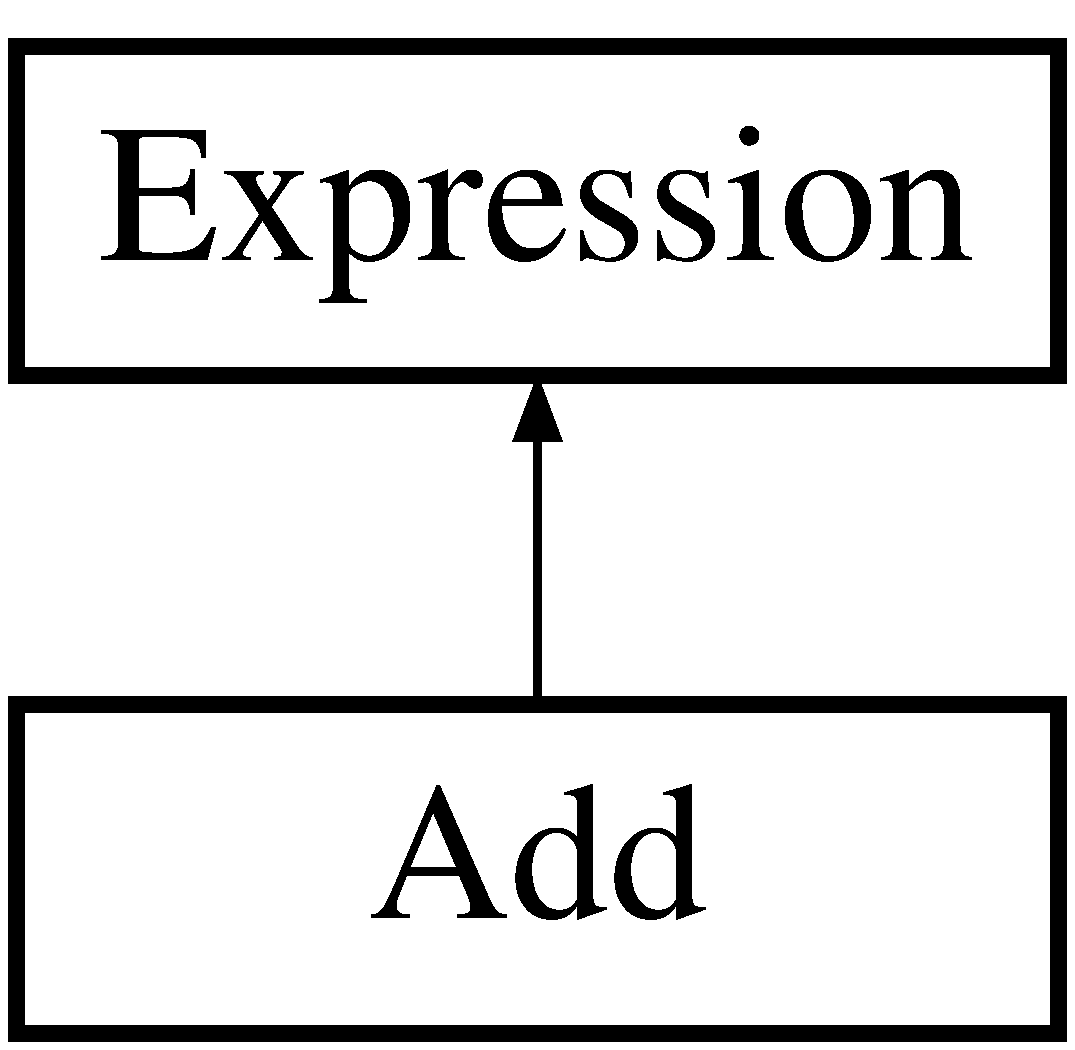
\includegraphics[height=2.000000cm]{class_add}
\end{center}
\end{figure}
\subsection*{Public Member Functions}
\begin{DoxyCompactItemize}
\item 
\hyperlink{class_add_aec3988b99721da89e8caa323f37c09f4}{Add} (\hyperlink{class_expression}{Expression} $\ast$lhs, \hyperlink{class_expression}{Expression} $\ast$rhs)
\begin{DoxyCompactList}\small\item\em Constructor method for the \hyperlink{class_add}{Add} class. \end{DoxyCompactList}\item 
\hyperlink{class_add_a960ca471ede083983766bce089f9af64}{$\sim$\+Add} ()
\begin{DoxyCompactList}\small\item\em Destructor method for the \hyperlink{class_add}{Add} class. \end{DoxyCompactList}\item 
virtual double \hyperlink{class_add_ac5b3425e7ac47b9f9a83e2f6da0d81ca}{evaluate} () const
\begin{DoxyCompactList}\small\item\em Adds the expressions together. \end{DoxyCompactList}\item 
virtual void \hyperlink{class_add_ad5af4ca57a44efab928c58ef39b00df1}{print} () const
\begin{DoxyCompactList}\small\item\em Prints out the addition. \end{DoxyCompactList}\end{DoxyCompactItemize}


\subsection{Detailed Description}
Addition expression. 

This Class serves as a representation of the \char`\"{}+\char`\"{} operation. 

\subsection{Constructor \& Destructor Documentation}
\mbox{\Hypertarget{class_add_aec3988b99721da89e8caa323f37c09f4}\label{class_add_aec3988b99721da89e8caa323f37c09f4}} 
\index{Add@{Add}!Add@{Add}}
\index{Add@{Add}!Add@{Add}}
\subsubsection{\texorpdfstring{Add()}{Add()}}
{\footnotesize\ttfamily Add\+::\+Add (\begin{DoxyParamCaption}\item[{\hyperlink{class_expression}{Expression} $\ast$}]{lhs,  }\item[{\hyperlink{class_expression}{Expression} $\ast$}]{rhs }\end{DoxyParamCaption})}



Constructor method for the \hyperlink{class_add}{Add} class. 

This constructor makes sure to initialize the left and right operands.


\begin{DoxyParams}{Parameters}
{\em lhs} & left hand side \hyperlink{class_expression}{Expression} \\
\hline
{\em rhs} & right hand side \hyperlink{class_expression}{Expression} \\
\hline
\end{DoxyParams}
\mbox{\Hypertarget{class_add_a960ca471ede083983766bce089f9af64}\label{class_add_a960ca471ede083983766bce089f9af64}} 
\index{Add@{Add}!````~Add@{$\sim$\+Add}}
\index{````~Add@{$\sim$\+Add}!Add@{Add}}
\subsubsection{\texorpdfstring{$\sim$\+Add()}{~Add()}}
{\footnotesize\ttfamily Add\+::$\sim$\+Add (\begin{DoxyParamCaption}{ }\end{DoxyParamCaption})}



Destructor method for the \hyperlink{class_add}{Add} class. 

This destructor deletes the expressions stored in the \hyperlink{class_add}{Add} Class and thus frees up the memory. 

\subsection{Member Function Documentation}
\mbox{\Hypertarget{class_add_ac5b3425e7ac47b9f9a83e2f6da0d81ca}\label{class_add_ac5b3425e7ac47b9f9a83e2f6da0d81ca}} 
\index{Add@{Add}!evaluate@{evaluate}}
\index{evaluate@{evaluate}!Add@{Add}}
\subsubsection{\texorpdfstring{evaluate()}{evaluate()}}
{\footnotesize\ttfamily double Add\+::evaluate (\begin{DoxyParamCaption}{ }\end{DoxyParamCaption}) const\hspace{0.3cm}{\ttfamily [virtual]}}



Adds the expressions together. 

This function adds the left and the right expressions together. They may be simple doubles or long expressions of the \hyperlink{class_expression}{Expression} datatype. This is why evaluation of both operands is needed before the addition operation can be performed, as to make sure to complete all the previous operations first.

\begin{DoxyReturn}{Returns}
The sum of the left and the right expressions 
\end{DoxyReturn}


Implements \hyperlink{class_expression_a7437adfabeaeb0500d62d10c43a1f853}{Expression}.

\mbox{\Hypertarget{class_add_ad5af4ca57a44efab928c58ef39b00df1}\label{class_add_ad5af4ca57a44efab928c58ef39b00df1}} 
\index{Add@{Add}!print@{print}}
\index{print@{print}!Add@{Add}}
\subsubsection{\texorpdfstring{print()}{print()}}
{\footnotesize\ttfamily void Add\+::print (\begin{DoxyParamCaption}{ }\end{DoxyParamCaption}) const\hspace{0.3cm}{\ttfamily [virtual]}}



Prints out the addition. 

This functions outputs the addition operation performed in a human readable fashion with brackets and a \char`\"{}+\char`\"{} symbol. 

Implements \hyperlink{class_expression_a6e05f883ebf77faf344dbaebfc82b3a0}{Expression}.



The documentation for this class was generated from the following files\+:\begin{DoxyCompactItemize}
\item 
\hyperlink{add_8h}{add.\+h}\item 
\hyperlink{add_8cpp}{add.\+cpp}\end{DoxyCompactItemize}

\hypertarget{class_const}{}\section{Const Class Reference}
\label{class_const}\index{Const@{Const}}


Saves a value for further calculation.  




{\ttfamily \#include $<$const.\+h$>$}

Inheritance diagram for Const\+:\begin{figure}[H]
\begin{center}
\leavevmode
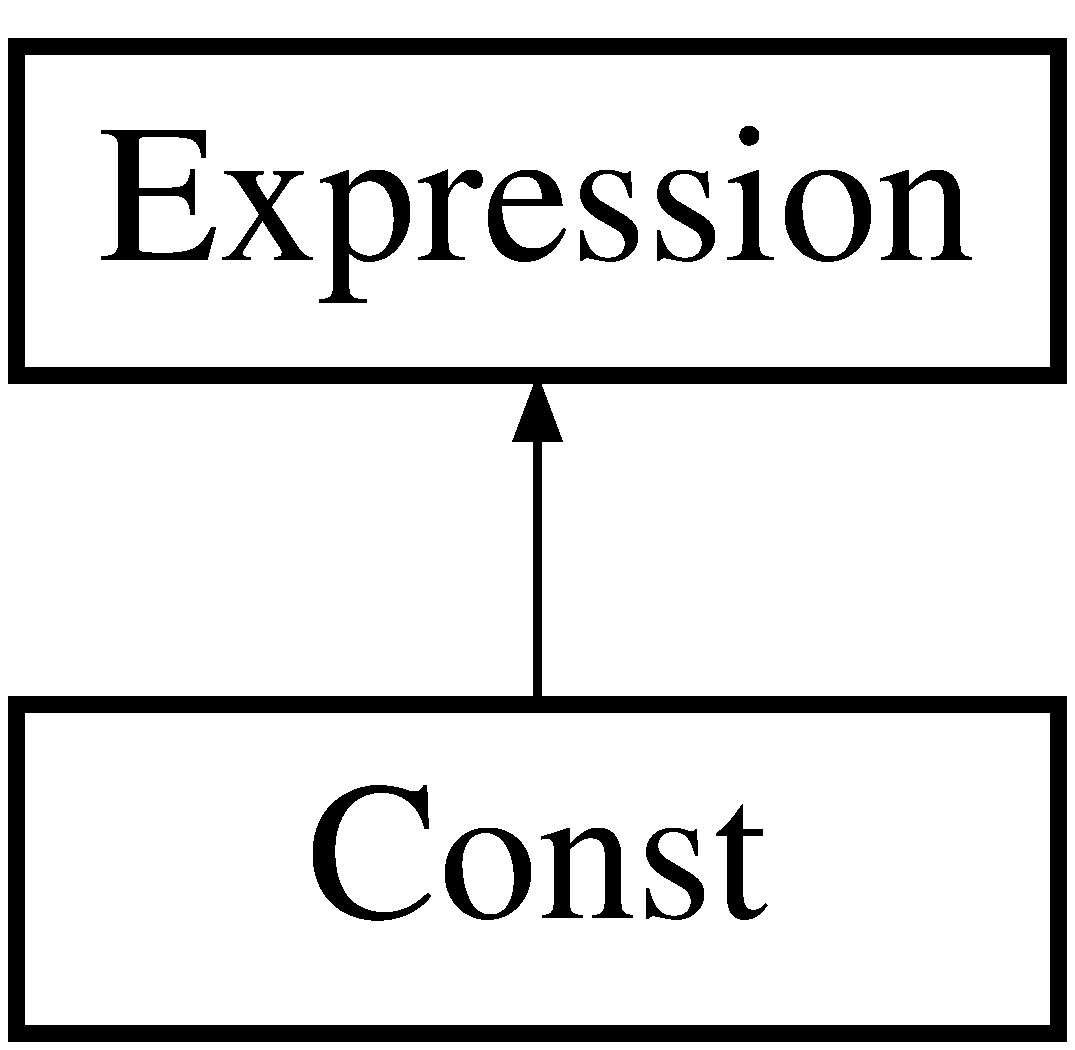
\includegraphics[height=2.000000cm]{class_const}
\end{center}
\end{figure}
\subsection*{Public Member Functions}
\begin{DoxyCompactItemize}
\item 
\hyperlink{class_const_a0d12dfb3f9b2ada576ce78d4914227ad}{Const} (double initval)
\begin{DoxyCompactList}\small\item\em Constuctor method for \hyperlink{class_const}{Const} Class. \end{DoxyCompactList}\item 
\mbox{\Hypertarget{class_const_a458fd0ff9671ebb6bba2e54247753126}\label{class_const_a458fd0ff9671ebb6bba2e54247753126}} 
\hyperlink{class_const_a458fd0ff9671ebb6bba2e54247753126}{$\sim$\+Const} ()
\begin{DoxyCompactList}\small\item\em Destructor method for \hyperlink{class_const}{Const} Class. \end{DoxyCompactList}\item 
double \hyperlink{class_const_a2f86d9af4cbc9dda466815c66360ba16}{evaluate} () const
\begin{DoxyCompactList}\small\item\em Polymorphous Evaluate method for \hyperlink{class_const}{Const} Class. \end{DoxyCompactList}\item 
\mbox{\Hypertarget{class_const_a81dc57c45d716e31d1cdb65a2c8f227d}\label{class_const_a81dc57c45d716e31d1cdb65a2c8f227d}} 
virtual void \hyperlink{class_const_a81dc57c45d716e31d1cdb65a2c8f227d}{print} () const
\begin{DoxyCompactList}\small\item\em Polymorphous Print method for \hyperlink{class_const}{Const} Class. \end{DoxyCompactList}\end{DoxyCompactItemize}


\subsection{Detailed Description}
Saves a value for further calculation. 

This Class saves a value inside its private \char`\"{}value\char`\"{} variable 

\subsection{Constructor \& Destructor Documentation}
\mbox{\Hypertarget{class_const_a0d12dfb3f9b2ada576ce78d4914227ad}\label{class_const_a0d12dfb3f9b2ada576ce78d4914227ad}} 
\index{Const@{Const}!Const@{Const}}
\index{Const@{Const}!Const@{Const}}
\subsubsection{\texorpdfstring{Const()}{Const()}}
{\footnotesize\ttfamily Const\+::\+Const (\begin{DoxyParamCaption}\item[{double}]{initval }\end{DoxyParamCaption})}



Constuctor method for \hyperlink{class_const}{Const} Class. 

This constructor initializes a \hyperlink{class_const}{Const} class instance with an integer value given to it that is then saved in it\textquotesingle{}s private variable \char`\"{}value\char`\"{}.


\begin{DoxyParams}{Parameters}
{\em initval} & The value with which it initializes \\
\hline
\end{DoxyParams}


\subsection{Member Function Documentation}
\mbox{\Hypertarget{class_const_a2f86d9af4cbc9dda466815c66360ba16}\label{class_const_a2f86d9af4cbc9dda466815c66360ba16}} 
\index{Const@{Const}!evaluate@{evaluate}}
\index{evaluate@{evaluate}!Const@{Const}}
\subsubsection{\texorpdfstring{evaluate()}{evaluate()}}
{\footnotesize\ttfamily double Const\+::evaluate (\begin{DoxyParamCaption}{ }\end{DoxyParamCaption}) const\hspace{0.3cm}{\ttfamily [virtual]}}



Polymorphous Evaluate method for \hyperlink{class_const}{Const} Class. 

\begin{DoxyReturn}{Returns}
double \hyperlink{class_result}{Result} of this expression 
\end{DoxyReturn}


Implements \hyperlink{class_expression_a7437adfabeaeb0500d62d10c43a1f853}{Expression}.



The documentation for this class was generated from the following files\+:\begin{DoxyCompactItemize}
\item 
\hyperlink{const_8h}{const.\+h}\item 
\hyperlink{const_8cpp}{const.\+cpp}\end{DoxyCompactItemize}

\hypertarget{class_div}{}\section{Div Class Reference}
\label{class_div}\index{Div@{Div}}


Division expression.  




{\ttfamily \#include $<$div.\+h$>$}

Inheritance diagram for Div\+:\begin{figure}[H]
\begin{center}
\leavevmode
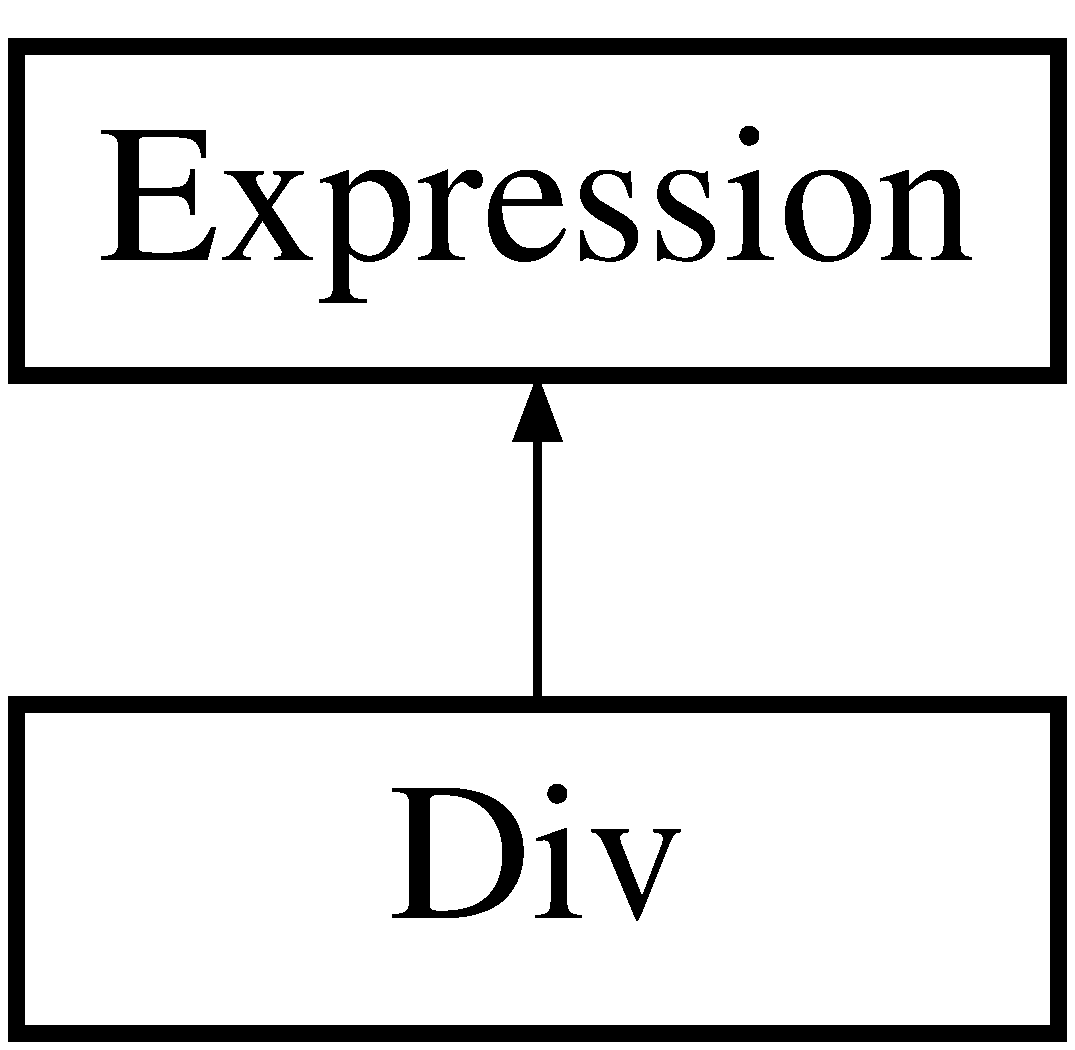
\includegraphics[height=2.000000cm]{class_div}
\end{center}
\end{figure}
\subsection*{Public Member Functions}
\begin{DoxyCompactItemize}
\item 
\hyperlink{class_div_a09066be0ef1596f1f673fe7a072cdc2d}{Div} (\hyperlink{class_expression}{Expression} $\ast$lhs, \hyperlink{class_expression}{Expression} $\ast$rhs)
\begin{DoxyCompactList}\small\item\em Constructor method for the \hyperlink{class_div}{Div} class. \end{DoxyCompactList}\item 
\hyperlink{class_div_ad4e297304eb13dfd034c9e0459ecfc4d}{$\sim$\+Div} ()
\begin{DoxyCompactList}\small\item\em Destructor method for the \hyperlink{class_div}{Div} class. \end{DoxyCompactList}\item 
virtual double \hyperlink{class_div_a5b96e19e7cffdb205a9e56377be3652e}{evaluate} () const
\begin{DoxyCompactList}\small\item\em Divides the expressions. \end{DoxyCompactList}\item 
virtual void \hyperlink{class_div_acbcc6e3d0f3ccb5e74de28de8499cbbf}{print} () const
\begin{DoxyCompactList}\small\item\em Prints out the product. \end{DoxyCompactList}\end{DoxyCompactItemize}


\subsection{Detailed Description}
Division expression. 

This Class serves as a representation of the \char`\"{}/\char`\"{} operation. 

\subsection{Constructor \& Destructor Documentation}
\mbox{\Hypertarget{class_div_a09066be0ef1596f1f673fe7a072cdc2d}\label{class_div_a09066be0ef1596f1f673fe7a072cdc2d}} 
\index{Div@{Div}!Div@{Div}}
\index{Div@{Div}!Div@{Div}}
\subsubsection{\texorpdfstring{Div()}{Div()}}
{\footnotesize\ttfamily Div\+::\+Div (\begin{DoxyParamCaption}\item[{\hyperlink{class_expression}{Expression} $\ast$}]{lhs,  }\item[{\hyperlink{class_expression}{Expression} $\ast$}]{rhs }\end{DoxyParamCaption})}



Constructor method for the \hyperlink{class_div}{Div} class. 

This constructor makes sure to initialize the left and right operands.


\begin{DoxyParams}{Parameters}
{\em lhs} & left hand side \hyperlink{class_expression}{Expression} \\
\hline
{\em rhs} & right hand side \hyperlink{class_expression}{Expression} \\
\hline
\end{DoxyParams}
\mbox{\Hypertarget{class_div_ad4e297304eb13dfd034c9e0459ecfc4d}\label{class_div_ad4e297304eb13dfd034c9e0459ecfc4d}} 
\index{Div@{Div}!````~Div@{$\sim$\+Div}}
\index{````~Div@{$\sim$\+Div}!Div@{Div}}
\subsubsection{\texorpdfstring{$\sim$\+Div()}{~Div()}}
{\footnotesize\ttfamily Div\+::$\sim$\+Div (\begin{DoxyParamCaption}{ }\end{DoxyParamCaption})}



Destructor method for the \hyperlink{class_div}{Div} class. 

This destructor deletes the expressions stored in the \hyperlink{class_div}{Div} Class and thus frees up the memory. 

\subsection{Member Function Documentation}
\mbox{\Hypertarget{class_div_a5b96e19e7cffdb205a9e56377be3652e}\label{class_div_a5b96e19e7cffdb205a9e56377be3652e}} 
\index{Div@{Div}!evaluate@{evaluate}}
\index{evaluate@{evaluate}!Div@{Div}}
\subsubsection{\texorpdfstring{evaluate()}{evaluate()}}
{\footnotesize\ttfamily double Div\+::evaluate (\begin{DoxyParamCaption}{ }\end{DoxyParamCaption}) const\hspace{0.3cm}{\ttfamily [virtual]}}



Divides the expressions. 

This function divides the left and the right expressions. They may be simple doubles or long expressions of the \hyperlink{class_expression}{Expression} datatype. This is why evaluation of both operands is needed before the division operation can be performed, as to make sure to complete all the previous operations first.

\begin{DoxyReturn}{Returns}
The quotient of the left and the right expressions 
\end{DoxyReturn}


Implements \hyperlink{class_expression_a7437adfabeaeb0500d62d10c43a1f853}{Expression}.

\mbox{\Hypertarget{class_div_acbcc6e3d0f3ccb5e74de28de8499cbbf}\label{class_div_acbcc6e3d0f3ccb5e74de28de8499cbbf}} 
\index{Div@{Div}!print@{print}}
\index{print@{print}!Div@{Div}}
\subsubsection{\texorpdfstring{print()}{print()}}
{\footnotesize\ttfamily void Div\+::print (\begin{DoxyParamCaption}{ }\end{DoxyParamCaption}) const\hspace{0.3cm}{\ttfamily [virtual]}}



Prints out the product. 

This functions outputs the multiplication operation performed in a human readable fashion with brackets and a \char`\"{}$\ast$\char`\"{} symbol. 

Implements \hyperlink{class_expression_a6e05f883ebf77faf344dbaebfc82b3a0}{Expression}.



The documentation for this class was generated from the following files\+:\begin{DoxyCompactItemize}
\item 
\hyperlink{div_8h}{div.\+h}\item 
\hyperlink{div_8cpp}{div.\+cpp}\end{DoxyCompactItemize}

\hypertarget{class_expression}{}\section{Expression Class Reference}
\label{class_expression}\index{Expression@{Expression}}


Abstract \hyperlink{class_expression}{Expression} Class.  




{\ttfamily \#include $<$expression.\+h$>$}

Inheritance diagram for Expression\+:\begin{figure}[H]
\begin{center}
\leavevmode
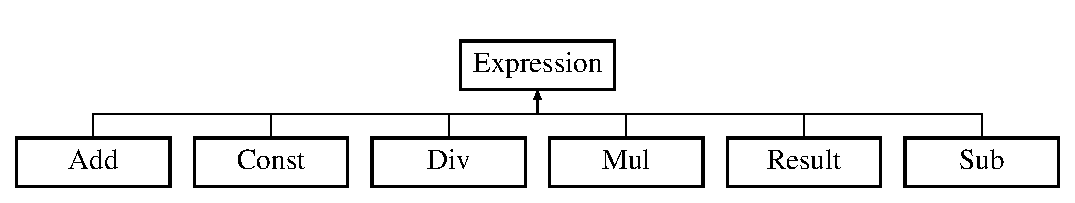
\includegraphics[height=2.000000cm]{class_expression}
\end{center}
\end{figure}
\subsection*{Public Member Functions}
\begin{DoxyCompactItemize}
\item 
\mbox{\Hypertarget{class_expression_afcf87716bf0abfe8d414c92529e1564a}\label{class_expression_afcf87716bf0abfe8d414c92529e1564a}} 
\hyperlink{class_expression_afcf87716bf0abfe8d414c92529e1564a}{Expression} ()
\begin{DoxyCompactList}\small\item\em Constructor method for \hyperlink{class_expression}{Expression} Class. \end{DoxyCompactList}\item 
\mbox{\Hypertarget{class_expression_a3e99570b177da619eeb2c5787cbb148e}\label{class_expression_a3e99570b177da619eeb2c5787cbb148e}} 
virtual \hyperlink{class_expression_a3e99570b177da619eeb2c5787cbb148e}{$\sim$\+Expression} ()
\begin{DoxyCompactList}\small\item\em Destructor method for \hyperlink{class_expression}{Expression} Class. \end{DoxyCompactList}\item 
virtual double \hyperlink{class_expression_a7437adfabeaeb0500d62d10c43a1f853}{evaluate} () const =0
\begin{DoxyCompactList}\small\item\em Calculates the expression. \end{DoxyCompactList}\item 
virtual void \hyperlink{class_expression_a6e05f883ebf77faf344dbaebfc82b3a0}{print} () const =0
\begin{DoxyCompactList}\small\item\em Prints the expression. \end{DoxyCompactList}\end{DoxyCompactItemize}


\subsection{Detailed Description}
Abstract \hyperlink{class_expression}{Expression} Class. 

This class is a parent for all the other implemented classes in this calculator. 

\subsection{Member Function Documentation}
\mbox{\Hypertarget{class_expression_a7437adfabeaeb0500d62d10c43a1f853}\label{class_expression_a7437adfabeaeb0500d62d10c43a1f853}} 
\index{Expression@{Expression}!evaluate@{evaluate}}
\index{evaluate@{evaluate}!Expression@{Expression}}
\subsubsection{\texorpdfstring{evaluate()}{evaluate()}}
{\footnotesize\ttfamily double Expression\+::evaluate (\begin{DoxyParamCaption}{ }\end{DoxyParamCaption}) const\hspace{0.3cm}{\ttfamily [pure virtual]}}



Calculates the expression. 

This function is the one actually calculation an expression.

\begin{DoxyReturn}{Returns}
Returns the calculation result 
\end{DoxyReturn}


Implemented in \hyperlink{class_const_a2f86d9af4cbc9dda466815c66360ba16}{Const}, \hyperlink{class_result_a107a060722c095f33008ca435cb2397d}{Result}, \hyperlink{class_add_ac5b3425e7ac47b9f9a83e2f6da0d81ca}{Add}, \hyperlink{class_div_a5b96e19e7cffdb205a9e56377be3652e}{Div}, \hyperlink{class_mul_a3e98f760d06aaac61dda9ab57d174a35}{Mul}, and \hyperlink{class_sub_a15b87b081136f533a993a92ac01ec11b}{Sub}.

\mbox{\Hypertarget{class_expression_a6e05f883ebf77faf344dbaebfc82b3a0}\label{class_expression_a6e05f883ebf77faf344dbaebfc82b3a0}} 
\index{Expression@{Expression}!print@{print}}
\index{print@{print}!Expression@{Expression}}
\subsubsection{\texorpdfstring{print()}{print()}}
{\footnotesize\ttfamily void Expression\+::print (\begin{DoxyParamCaption}{ }\end{DoxyParamCaption}) const\hspace{0.3cm}{\ttfamily [pure virtual]}}



Prints the expression. 

This function prints the currerntly calculated mathematical expression to the user in the most human-\/readable way possible. 

Implemented in \hyperlink{class_const_a81dc57c45d716e31d1cdb65a2c8f227d}{Const}, \hyperlink{class_result_a17227de791c97a6eee68689f4317cafa}{Result}, \hyperlink{class_add_ad5af4ca57a44efab928c58ef39b00df1}{Add}, \hyperlink{class_div_acbcc6e3d0f3ccb5e74de28de8499cbbf}{Div}, \hyperlink{class_mul_a0aa9276f2fc04dd9afc77bf47542e5ec}{Mul}, and \hyperlink{class_sub_a2e7c967c1fdee5e7eca51ca36feb26bc}{Sub}.



The documentation for this class was generated from the following files\+:\begin{DoxyCompactItemize}
\item 
\hyperlink{expression_8h}{expression.\+h}\item 
expression.\+cpp\end{DoxyCompactItemize}

\hypertarget{class_mul}{}\section{Mul Class Reference}
\label{class_mul}\index{Mul@{Mul}}


Multiplication expression.  




{\ttfamily \#include $<$mul.\+h$>$}

Inheritance diagram for Mul\+:\begin{figure}[H]
\begin{center}
\leavevmode
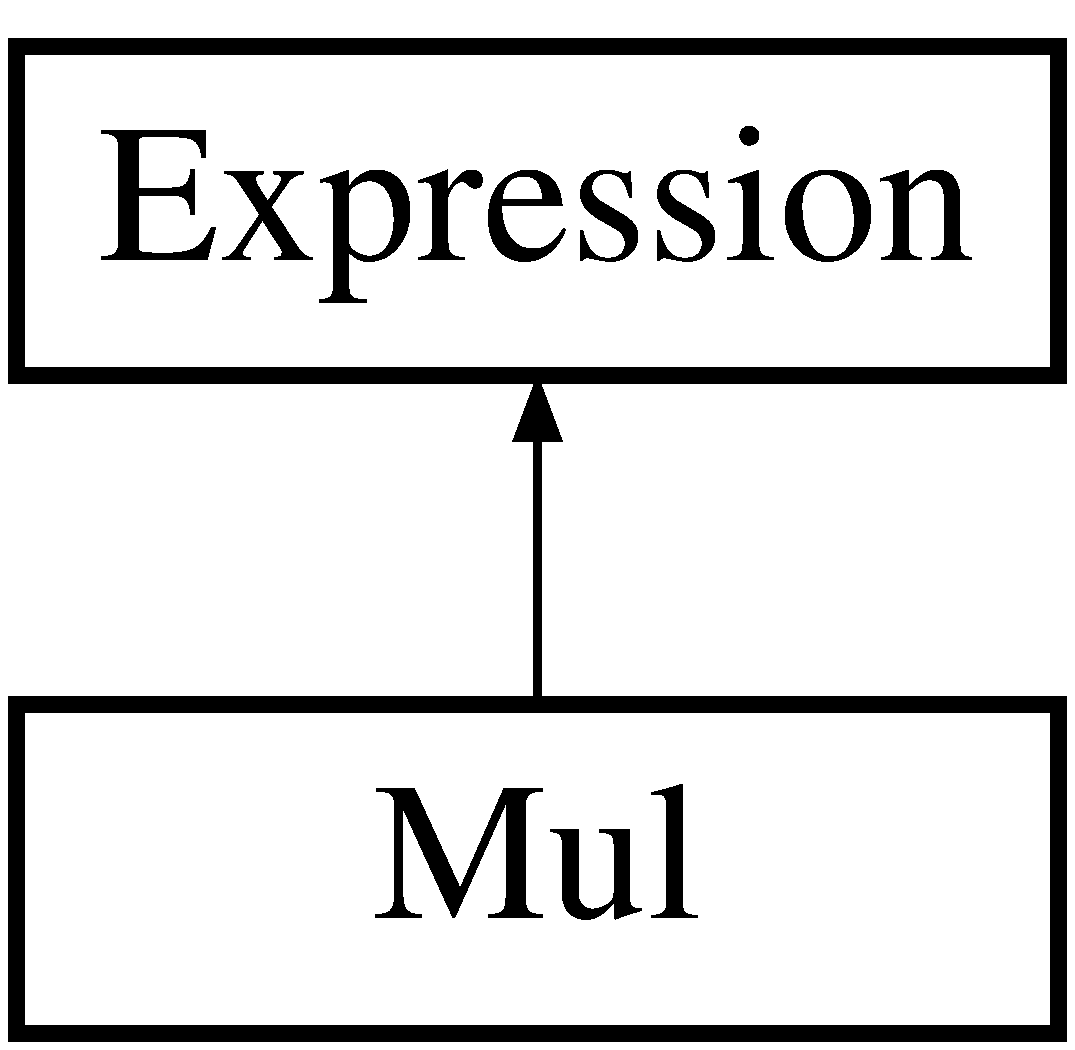
\includegraphics[height=2.000000cm]{class_mul}
\end{center}
\end{figure}
\subsection*{Public Member Functions}
\begin{DoxyCompactItemize}
\item 
\hyperlink{class_mul_af8f36e90eda7ce256bd1e93635d55750}{Mul} (\hyperlink{class_expression}{Expression} $\ast$lhs, \hyperlink{class_expression}{Expression} $\ast$rhs)
\begin{DoxyCompactList}\small\item\em Constructor method for the \hyperlink{class_mul}{Mul} class. \end{DoxyCompactList}\item 
\hyperlink{class_mul_ad072b4a8fa7c2c7acb794454d3b97c8c}{$\sim$\+Mul} ()
\begin{DoxyCompactList}\small\item\em Destructor method for the \hyperlink{class_mul}{Mul} class. \end{DoxyCompactList}\item 
virtual double \hyperlink{class_mul_a3e98f760d06aaac61dda9ab57d174a35}{evaluate} () const
\begin{DoxyCompactList}\small\item\em Multiplies the expressions. \end{DoxyCompactList}\item 
virtual void \hyperlink{class_mul_a0aa9276f2fc04dd9afc77bf47542e5ec}{print} () const
\begin{DoxyCompactList}\small\item\em Prints out the product. \end{DoxyCompactList}\end{DoxyCompactItemize}


\subsection{Detailed Description}
Multiplication expression. 

This Class serves as a representation of the \char`\"{}$\ast$\char`\"{} operation. 

\subsection{Constructor \& Destructor Documentation}
\mbox{\Hypertarget{class_mul_af8f36e90eda7ce256bd1e93635d55750}\label{class_mul_af8f36e90eda7ce256bd1e93635d55750}} 
\index{Mul@{Mul}!Mul@{Mul}}
\index{Mul@{Mul}!Mul@{Mul}}
\subsubsection{\texorpdfstring{Mul()}{Mul()}}
{\footnotesize\ttfamily Mul\+::\+Mul (\begin{DoxyParamCaption}\item[{\hyperlink{class_expression}{Expression} $\ast$}]{lhs,  }\item[{\hyperlink{class_expression}{Expression} $\ast$}]{rhs }\end{DoxyParamCaption})}



Constructor method for the \hyperlink{class_mul}{Mul} class. 

This constructor makes sure to initialize the left and right operands.


\begin{DoxyParams}{Parameters}
{\em lhs} & left hand side \hyperlink{class_expression}{Expression} \\
\hline
{\em rhs} & right hand side \hyperlink{class_expression}{Expression} \\
\hline
\end{DoxyParams}
\mbox{\Hypertarget{class_mul_ad072b4a8fa7c2c7acb794454d3b97c8c}\label{class_mul_ad072b4a8fa7c2c7acb794454d3b97c8c}} 
\index{Mul@{Mul}!````~Mul@{$\sim$\+Mul}}
\index{````~Mul@{$\sim$\+Mul}!Mul@{Mul}}
\subsubsection{\texorpdfstring{$\sim$\+Mul()}{~Mul()}}
{\footnotesize\ttfamily Mul\+::$\sim$\+Mul (\begin{DoxyParamCaption}{ }\end{DoxyParamCaption})}



Destructor method for the \hyperlink{class_mul}{Mul} class. 

This destructor deletes the expressions stored in the \hyperlink{class_mul}{Mul} Class and thus frees up the memory. 

\subsection{Member Function Documentation}
\mbox{\Hypertarget{class_mul_a3e98f760d06aaac61dda9ab57d174a35}\label{class_mul_a3e98f760d06aaac61dda9ab57d174a35}} 
\index{Mul@{Mul}!evaluate@{evaluate}}
\index{evaluate@{evaluate}!Mul@{Mul}}
\subsubsection{\texorpdfstring{evaluate()}{evaluate()}}
{\footnotesize\ttfamily double Mul\+::evaluate (\begin{DoxyParamCaption}{ }\end{DoxyParamCaption}) const\hspace{0.3cm}{\ttfamily [virtual]}}



Multiplies the expressions. 

This function multiplies the left and the right expressions. They may be simple doubles or long expressions of the \hyperlink{class_expression}{Expression} datatype. This is why evaluation of both operands is needed before the multiplication operation can be performed, as to make sure to complete all the previous operations first.

\begin{DoxyReturn}{Returns}
The product of the left and the right expressions 
\end{DoxyReturn}


Implements \hyperlink{class_expression_a7437adfabeaeb0500d62d10c43a1f853}{Expression}.

\mbox{\Hypertarget{class_mul_a0aa9276f2fc04dd9afc77bf47542e5ec}\label{class_mul_a0aa9276f2fc04dd9afc77bf47542e5ec}} 
\index{Mul@{Mul}!print@{print}}
\index{print@{print}!Mul@{Mul}}
\subsubsection{\texorpdfstring{print()}{print()}}
{\footnotesize\ttfamily void Mul\+::print (\begin{DoxyParamCaption}{ }\end{DoxyParamCaption}) const\hspace{0.3cm}{\ttfamily [virtual]}}



Prints out the product. 

This functions outputs the multiplication operation performed in a human readable fashion with brackets and a \char`\"{}$\ast$\char`\"{} symbol. 

Implements \hyperlink{class_expression_a6e05f883ebf77faf344dbaebfc82b3a0}{Expression}.



The documentation for this class was generated from the following files\+:\begin{DoxyCompactItemize}
\item 
\hyperlink{mul_8h}{mul.\+h}\item 
\hyperlink{mul_8cpp}{mul.\+cpp}\end{DoxyCompactItemize}

\hypertarget{class_result}{}\section{Result Class Reference}
\label{class_result}\index{Result@{Result}}


Calculates and saves the result.  




{\ttfamily \#include $<$result.\+h$>$}

Inheritance diagram for Result\+:\begin{figure}[H]
\begin{center}
\leavevmode
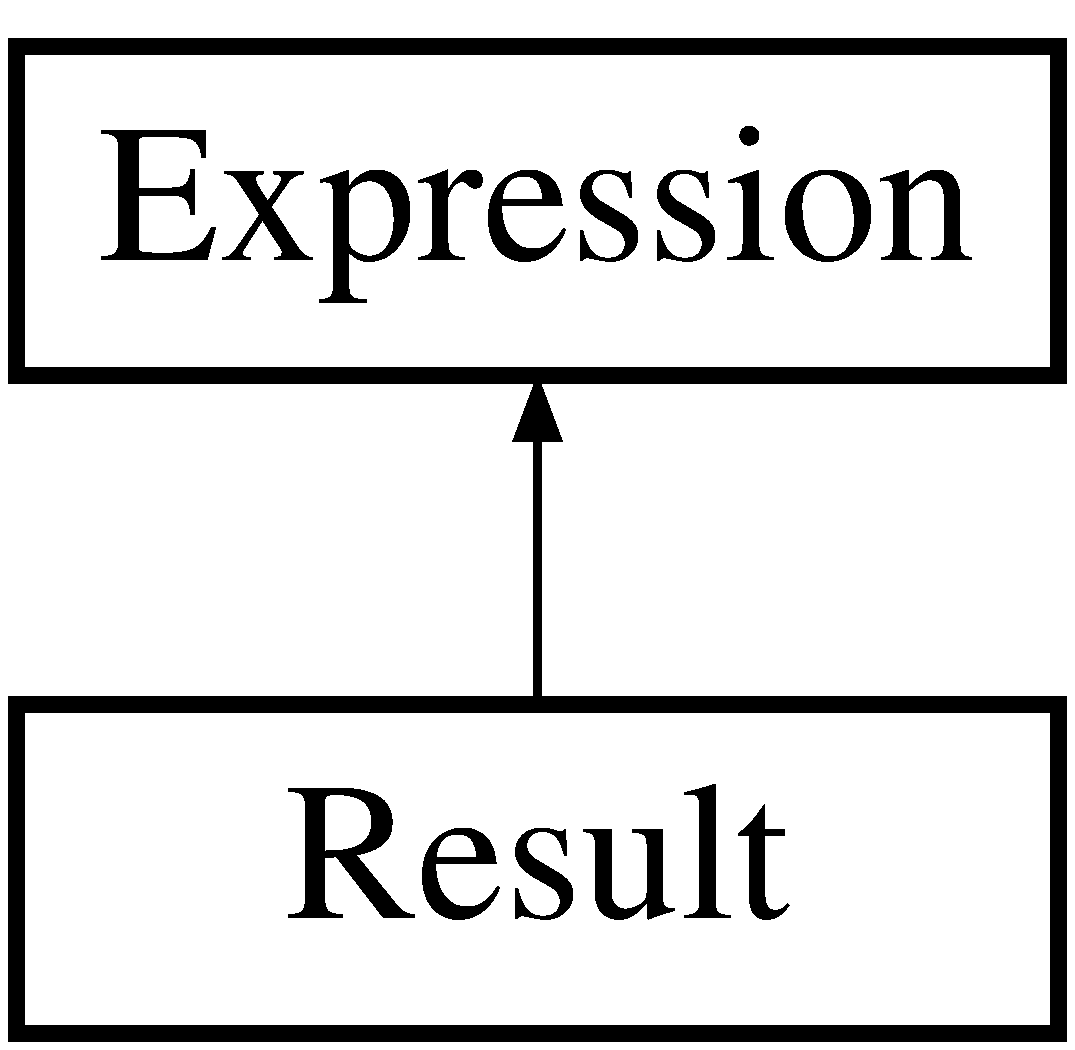
\includegraphics[height=2.000000cm]{class_result}
\end{center}
\end{figure}
\subsection*{Public Member Functions}
\begin{DoxyCompactItemize}
\item 
\mbox{\Hypertarget{class_result_aab8976a9cb715f82a3a28dea71882f04}\label{class_result_aab8976a9cb715f82a3a28dea71882f04}} 
\hyperlink{class_result_aab8976a9cb715f82a3a28dea71882f04}{Result} (\hyperlink{class_expression}{Expression} $\ast$currexpr)
\begin{DoxyCompactList}\small\item\em Constuctor for \hyperlink{class_result}{Result} Class. \end{DoxyCompactList}\item 
\mbox{\Hypertarget{class_result_ab83cf33a31236b3da75d66aaf9a05ed0}\label{class_result_ab83cf33a31236b3da75d66aaf9a05ed0}} 
\hyperlink{class_result_ab83cf33a31236b3da75d66aaf9a05ed0}{$\sim$\+Result} ()
\begin{DoxyCompactList}\small\item\em Destructor for \hyperlink{class_result}{Result} Class. \end{DoxyCompactList}\item 
\mbox{\Hypertarget{class_result_a107a060722c095f33008ca435cb2397d}\label{class_result_a107a060722c095f33008ca435cb2397d}} 
virtual double \hyperlink{class_result_a107a060722c095f33008ca435cb2397d}{evaluate} () const
\begin{DoxyCompactList}\small\item\em Polymorphous evaluate method for \hyperlink{class_result}{Result} Class. \end{DoxyCompactList}\item 
\mbox{\Hypertarget{class_result_a17227de791c97a6eee68689f4317cafa}\label{class_result_a17227de791c97a6eee68689f4317cafa}} 
virtual void \hyperlink{class_result_a17227de791c97a6eee68689f4317cafa}{print} () const
\begin{DoxyCompactList}\small\item\em Polymorphous print method for \hyperlink{class_result}{Result} Class. \end{DoxyCompactList}\end{DoxyCompactItemize}


\subsection{Detailed Description}
Calculates and saves the result. 

This Class is implemented to evaluate an expression and forward the result to the next operation, if such exists. 

The documentation for this class was generated from the following files\+:\begin{DoxyCompactItemize}
\item 
\hyperlink{result_8h}{result.\+h}\item 
\hyperlink{result_8cpp}{result.\+cpp}\end{DoxyCompactItemize}

\hypertarget{class_sub}{}\section{Sub Class Reference}
\label{class_sub}\index{Sub@{Sub}}


Subtraction expression.  




{\ttfamily \#include $<$sub.\+h$>$}

Inheritance diagram for Sub\+:\begin{figure}[H]
\begin{center}
\leavevmode
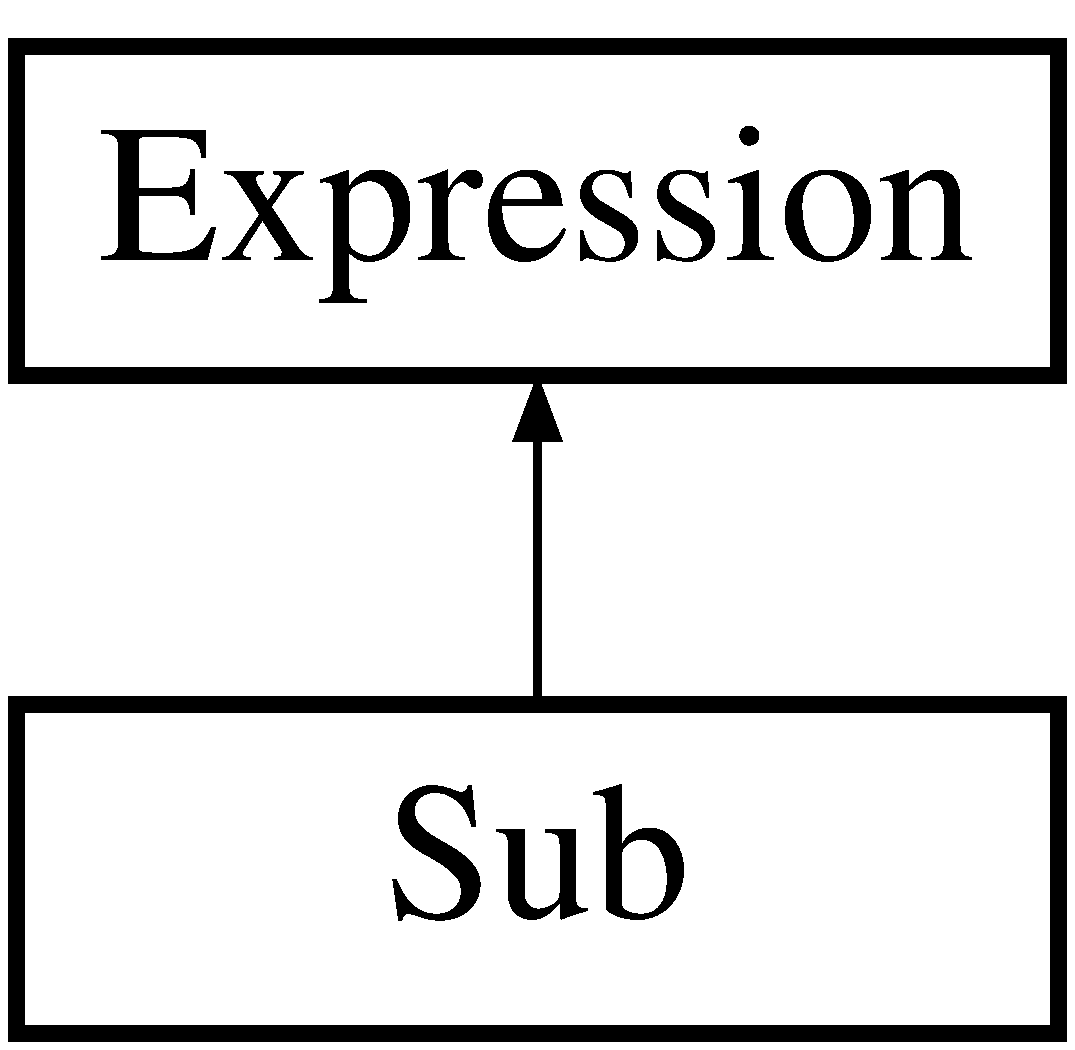
\includegraphics[height=2.000000cm]{class_sub}
\end{center}
\end{figure}
\subsection*{Public Member Functions}
\begin{DoxyCompactItemize}
\item 
\hyperlink{class_sub_a546d43098de078f66bc615544770133e}{Sub} (\hyperlink{class_expression}{Expression} $\ast$lhs, \hyperlink{class_expression}{Expression} $\ast$rhs)
\begin{DoxyCompactList}\small\item\em Constructor method for the \hyperlink{class_sub}{Sub} class. \end{DoxyCompactList}\item 
\hyperlink{class_sub_a01d5069c4d640cc4e6016a4794e435a5}{$\sim$\+Sub} ()
\begin{DoxyCompactList}\small\item\em Destructor method for the \hyperlink{class_mul}{Mul} class. \end{DoxyCompactList}\item 
virtual double \hyperlink{class_sub_a15b87b081136f533a993a92ac01ec11b}{evaluate} () const
\begin{DoxyCompactList}\small\item\em Subtracts the expressions. \end{DoxyCompactList}\item 
virtual void \hyperlink{class_sub_a2e7c967c1fdee5e7eca51ca36feb26bc}{print} () const
\begin{DoxyCompactList}\small\item\em Prints out the difference. \end{DoxyCompactList}\end{DoxyCompactItemize}


\subsection{Detailed Description}
Subtraction expression. 

This Class serves as a representation of the \char`\"{}-\/\char`\"{} operation. 

\subsection{Constructor \& Destructor Documentation}
\mbox{\Hypertarget{class_sub_a546d43098de078f66bc615544770133e}\label{class_sub_a546d43098de078f66bc615544770133e}} 
\index{Sub@{Sub}!Sub@{Sub}}
\index{Sub@{Sub}!Sub@{Sub}}
\subsubsection{\texorpdfstring{Sub()}{Sub()}}
{\footnotesize\ttfamily Sub\+::\+Sub (\begin{DoxyParamCaption}\item[{\hyperlink{class_expression}{Expression} $\ast$}]{lhs,  }\item[{\hyperlink{class_expression}{Expression} $\ast$}]{rhs }\end{DoxyParamCaption})}



Constructor method for the \hyperlink{class_sub}{Sub} class. 

This constructor makes sure to initialize the left and right operands.


\begin{DoxyParams}{Parameters}
{\em lhs} & left hand side \hyperlink{class_expression}{Expression} \\
\hline
{\em rhs} & right hand side \hyperlink{class_expression}{Expression} \\
\hline
\end{DoxyParams}
\mbox{\Hypertarget{class_sub_a01d5069c4d640cc4e6016a4794e435a5}\label{class_sub_a01d5069c4d640cc4e6016a4794e435a5}} 
\index{Sub@{Sub}!````~Sub@{$\sim$\+Sub}}
\index{````~Sub@{$\sim$\+Sub}!Sub@{Sub}}
\subsubsection{\texorpdfstring{$\sim$\+Sub()}{~Sub()}}
{\footnotesize\ttfamily Sub\+::$\sim$\+Sub (\begin{DoxyParamCaption}{ }\end{DoxyParamCaption})}



Destructor method for the \hyperlink{class_mul}{Mul} class. 

This destructor deletes the expressions stored in the \hyperlink{class_mul}{Mul} Class and thus frees up the memory. 

\subsection{Member Function Documentation}
\mbox{\Hypertarget{class_sub_a15b87b081136f533a993a92ac01ec11b}\label{class_sub_a15b87b081136f533a993a92ac01ec11b}} 
\index{Sub@{Sub}!evaluate@{evaluate}}
\index{evaluate@{evaluate}!Sub@{Sub}}
\subsubsection{\texorpdfstring{evaluate()}{evaluate()}}
{\footnotesize\ttfamily double Sub\+::evaluate (\begin{DoxyParamCaption}{ }\end{DoxyParamCaption}) const\hspace{0.3cm}{\ttfamily [virtual]}}



Subtracts the expressions. 

This function subtracts the right expression from the and the left one. They may be simple doubles or long expressions of the \hyperlink{class_expression}{Expression} datatype. This is why evaluation of both operands is needed before the subtraction operation can be performed, as to make sure to complete all the previous operations first.

\begin{DoxyReturn}{Returns}
The difference of the left and the right expressions 
\end{DoxyReturn}


Implements \hyperlink{class_expression_a7437adfabeaeb0500d62d10c43a1f853}{Expression}.

\mbox{\Hypertarget{class_sub_a2e7c967c1fdee5e7eca51ca36feb26bc}\label{class_sub_a2e7c967c1fdee5e7eca51ca36feb26bc}} 
\index{Sub@{Sub}!print@{print}}
\index{print@{print}!Sub@{Sub}}
\subsubsection{\texorpdfstring{print()}{print()}}
{\footnotesize\ttfamily void Sub\+::print (\begin{DoxyParamCaption}{ }\end{DoxyParamCaption}) const\hspace{0.3cm}{\ttfamily [virtual]}}



Prints out the difference. 

This functions outputs the subtraction operation performed in a human readable fashion with brackets and a \char`\"{}-\/\char`\"{} symbol. 

Implements \hyperlink{class_expression_a6e05f883ebf77faf344dbaebfc82b3a0}{Expression}.



The documentation for this class was generated from the following files\+:\begin{DoxyCompactItemize}
\item 
\hyperlink{sub_8h}{sub.\+h}\item 
\hyperlink{sub_8cpp}{sub.\+cpp}\end{DoxyCompactItemize}

\chapter{File Documentation}
\hypertarget{add_8cpp}{}\section{add.\+cpp File Reference}
\label{add_8cpp}\index{add.\+cpp@{add.\+cpp}}


Contains the method declarations used in the \hyperlink{class_add}{Add} Class.  


{\ttfamily \#include \char`\"{}add.\+h\char`\"{}}\newline
{\ttfamily \#include $<$iostream$>$}\newline


\subsection{Detailed Description}
Contains the method declarations used in the \hyperlink{class_add}{Add} Class. 


\hypertarget{add_8h}{}\section{add.\+h File Reference}
\label{add_8h}\index{add.\+h@{add.\+h}}


Header file for the \hyperlink{class_add}{Add} Class.  


{\ttfamily \#include \char`\"{}expression.\+h\char`\"{}}\newline
\subsection*{Classes}
\begin{DoxyCompactItemize}
\item 
class \hyperlink{class_add}{Add}
\begin{DoxyCompactList}\small\item\em Addition expression. \end{DoxyCompactList}\end{DoxyCompactItemize}


\subsection{Detailed Description}
Header file for the \hyperlink{class_add}{Add} Class. 


\hypertarget{const_8cpp}{}\section{const.\+cpp File Reference}
\label{const_8cpp}\index{const.\+cpp@{const.\+cpp}}


Contains the method declarations used in the \hyperlink{class_const}{Const} Class.  


{\ttfamily \#include $<$iostream$>$}\newline
{\ttfamily \#include \char`\"{}const.\+h\char`\"{}}\newline


\subsection{Detailed Description}
Contains the method declarations used in the \hyperlink{class_const}{Const} Class. 


\hypertarget{const_8h}{}\section{const.\+h File Reference}
\label{const_8h}\index{const.\+h@{const.\+h}}


Header file for the \hyperlink{class_const}{Const} Class.  


{\ttfamily \#include \char`\"{}expression.\+h\char`\"{}}\newline
\subsection*{Classes}
\begin{DoxyCompactItemize}
\item 
class \hyperlink{class_const}{Const}
\begin{DoxyCompactList}\small\item\em Saves a value for further calculation. \end{DoxyCompactList}\end{DoxyCompactItemize}


\subsection{Detailed Description}
Header file for the \hyperlink{class_const}{Const} Class. 


\hypertarget{div_8cpp}{}\section{div.\+cpp File Reference}
\label{div_8cpp}\index{div.\+cpp@{div.\+cpp}}


Contains the method declarations used in the \hyperlink{class_div}{Div} Class.  


{\ttfamily \#include $<$iostream$>$}\newline
{\ttfamily \#include \char`\"{}div.\+h\char`\"{}}\newline


\subsection{Detailed Description}
Contains the method declarations used in the \hyperlink{class_div}{Div} Class. 


\hypertarget{div_8h}{}\section{div.\+h File Reference}
\label{div_8h}\index{div.\+h@{div.\+h}}


Header file for the \hyperlink{class_div}{Div} Class.  


{\ttfamily \#include \char`\"{}expression.\+h\char`\"{}}\newline
\subsection*{Classes}
\begin{DoxyCompactItemize}
\item 
class \hyperlink{class_div}{Div}
\begin{DoxyCompactList}\small\item\em Division expression. \end{DoxyCompactList}\end{DoxyCompactItemize}


\subsection{Detailed Description}
Header file for the \hyperlink{class_div}{Div} Class. 


\hypertarget{expression_8h}{}\section{expression.\+h File Reference}
\label{expression_8h}\index{expression.\+h@{expression.\+h}}


Header file for the \hyperlink{class_expression}{Expression} Class.  


\subsection*{Classes}
\begin{DoxyCompactItemize}
\item 
class \hyperlink{class_expression}{Expression}
\begin{DoxyCompactList}\small\item\em Abstract \hyperlink{class_expression}{Expression} Class. \end{DoxyCompactList}\end{DoxyCompactItemize}


\subsection{Detailed Description}
Header file for the \hyperlink{class_expression}{Expression} Class. 

Praktikum Informatik 1 M\+M\+X\+V\+II Versuch 8\+: Taschenrechner

Datei\+: \hyperlink{expression_8h}{expression.\+h} Inhalt\+: Headerdatei Abstrakte Klasse \hyperlink{class_expression}{Expression} 
\hypertarget{mul_8cpp}{}\section{mul.\+cpp File Reference}
\label{mul_8cpp}\index{mul.\+cpp@{mul.\+cpp}}


Contains the method declarations used in the \hyperlink{class_mul}{Mul} Class.  


{\ttfamily \#include $<$iostream$>$}\newline
{\ttfamily \#include \char`\"{}mul.\+h\char`\"{}}\newline


\subsection{Detailed Description}
Contains the method declarations used in the \hyperlink{class_mul}{Mul} Class. 


\hypertarget{mul_8h}{}\section{mul.\+h File Reference}
\label{mul_8h}\index{mul.\+h@{mul.\+h}}


Header file for the \hyperlink{class_mul}{Mul} Class.  


{\ttfamily \#include \char`\"{}expression.\+h\char`\"{}}\newline
\subsection*{Classes}
\begin{DoxyCompactItemize}
\item 
class \hyperlink{class_mul}{Mul}
\begin{DoxyCompactList}\small\item\em Multiplication expression. \end{DoxyCompactList}\end{DoxyCompactItemize}


\subsection{Detailed Description}
Header file for the \hyperlink{class_mul}{Mul} Class. 


\hypertarget{result_8cpp}{}\section{result.\+cpp File Reference}
\label{result_8cpp}\index{result.\+cpp@{result.\+cpp}}


Contains the method declarations used in the \hyperlink{class_result}{Result} Class.  


{\ttfamily \#include $<$iostream$>$}\newline
{\ttfamily \#include \char`\"{}result.\+h\char`\"{}}\newline


\subsection{Detailed Description}
Contains the method declarations used in the \hyperlink{class_result}{Result} Class. 


\hypertarget{result_8h}{}\section{result.\+h File Reference}
\label{result_8h}\index{result.\+h@{result.\+h}}


Header file for the \hyperlink{class_result}{Result} Class.  


{\ttfamily \#include \char`\"{}expression.\+h\char`\"{}}\newline
\subsection*{Classes}
\begin{DoxyCompactItemize}
\item 
class \hyperlink{class_result}{Result}
\begin{DoxyCompactList}\small\item\em Calculates and saves the result. \end{DoxyCompactList}\end{DoxyCompactItemize}


\subsection{Detailed Description}
Header file for the \hyperlink{class_result}{Result} Class. 


\hypertarget{sub_8cpp}{}\section{sub.\+cpp File Reference}
\label{sub_8cpp}\index{sub.\+cpp@{sub.\+cpp}}


Contains the method declarations used in the \hyperlink{class_sub}{Sub} Class.  


{\ttfamily \#include $<$iostream$>$}\newline
{\ttfamily \#include \char`\"{}sub.\+h\char`\"{}}\newline


\subsection{Detailed Description}
Contains the method declarations used in the \hyperlink{class_sub}{Sub} Class. 


\hypertarget{sub_8h}{}\section{sub.\+h File Reference}
\label{sub_8h}\index{sub.\+h@{sub.\+h}}


Header file for the \hyperlink{class_sub}{Sub} Class.  


{\ttfamily \#include \char`\"{}expression.\+h\char`\"{}}\newline
\subsection*{Classes}
\begin{DoxyCompactItemize}
\item 
class \hyperlink{class_sub}{Sub}
\begin{DoxyCompactList}\small\item\em Subtraction expression. \end{DoxyCompactList}\end{DoxyCompactItemize}


\subsection{Detailed Description}
Header file for the \hyperlink{class_sub}{Sub} Class. 


\hypertarget{taschenrechner_8cpp}{}\section{taschenrechner.\+cpp File Reference}
\label{taschenrechner_8cpp}\index{taschenrechner.\+cpp@{taschenrechner.\+cpp}}


Main Routine Datei\+: \hyperlink{taschenrechner_8cpp}{taschenrechner.\+cpp} Inhalt\+: Hauptprogramm.  


{\ttfamily \#include $<$iostream$>$}\newline
{\ttfamily \#include \char`\"{}expression.\+h\char`\"{}}\newline
{\ttfamily \#include \char`\"{}const.\+h\char`\"{}}\newline
{\ttfamily \#include \char`\"{}result.\+h\char`\"{}}\newline
{\ttfamily \#include \char`\"{}add.\+h\char`\"{}}\newline
{\ttfamily \#include \char`\"{}mul.\+h\char`\"{}}\newline
{\ttfamily \#include \char`\"{}sub.\+h\char`\"{}}\newline
{\ttfamily \#include \char`\"{}div.\+h\char`\"{}}\newline
\subsection*{Functions}
\begin{DoxyCompactItemize}
\item 
void \hyperlink{taschenrechner_8cpp_a980e2b5b40f379d5bbe4cc9157a250b3}{test\+Const} ()
\begin{DoxyCompactList}\small\item\em Test function for the \hyperlink{class_const}{Const} Class. \end{DoxyCompactList}\item 
void \hyperlink{taschenrechner_8cpp_a18aad0c82633c7449592bfe1dc739f60}{test\+Result} ()
\begin{DoxyCompactList}\small\item\em Test function for the \hyperlink{class_result}{Result} Class. \end{DoxyCompactList}\item 
void \hyperlink{taschenrechner_8cpp_aaf2b23089f5910c3ca27b72e91b89603}{test\+Add\+Const} ()
\begin{DoxyCompactList}\small\item\em Test function for the \hyperlink{class_add}{Add} Class. \end{DoxyCompactList}\item 
void \hyperlink{taschenrechner_8cpp_a986ee1802fe96dd6fe908c0602634321}{test\+Mul\+Add\+Const} ()
\begin{DoxyCompactList}\small\item\em Test function for the \hyperlink{class_add}{Add} Class and \hyperlink{class_mul}{Mul} Class together. \end{DoxyCompactList}\item 
void \hyperlink{taschenrechner_8cpp_a9eadd474e616fa432dd725cc8161c495}{test\+Sub\+Mul\+Add\+Const} ()
\begin{DoxyCompactList}\small\item\em Test function for the \hyperlink{class_sub}{Sub}, \hyperlink{class_mul}{Mul} and \hyperlink{class_add}{Add} Classes. \end{DoxyCompactList}\item 
void \hyperlink{taschenrechner_8cpp_a49cc1f74374f4441d9faf5b7d96072f2}{final\+Test} ()
\begin{DoxyCompactList}\small\item\em Final general test. \end{DoxyCompactList}\item 
\mbox{\Hypertarget{taschenrechner_8cpp_ae66f6b31b5ad750f1fe042a706a4e3d4}\label{taschenrechner_8cpp_ae66f6b31b5ad750f1fe042a706a4e3d4}} 
int \hyperlink{taschenrechner_8cpp_ae66f6b31b5ad750f1fe042a706a4e3d4}{main} ()
\begin{DoxyCompactList}\small\item\em Main routine. \end{DoxyCompactList}\end{DoxyCompactItemize}


\subsection{Detailed Description}
Main Routine Datei\+: \hyperlink{taschenrechner_8cpp}{taschenrechner.\+cpp} Inhalt\+: Hauptprogramm. 

\begin{DoxyAuthor}{Author}
Can Oezmaden 
\end{DoxyAuthor}
\begin{DoxyDate}{Date}
Juli 2017 
\end{DoxyDate}


\subsection{Function Documentation}
\mbox{\Hypertarget{taschenrechner_8cpp_a49cc1f74374f4441d9faf5b7d96072f2}\label{taschenrechner_8cpp_a49cc1f74374f4441d9faf5b7d96072f2}} 
\index{taschenrechner.\+cpp@{taschenrechner.\+cpp}!final\+Test@{final\+Test}}
\index{final\+Test@{final\+Test}!taschenrechner.\+cpp@{taschenrechner.\+cpp}}
\subsubsection{\texorpdfstring{final\+Test()}{finalTest()}}
{\footnotesize\ttfamily void final\+Test (\begin{DoxyParamCaption}{ }\end{DoxyParamCaption})}



Final general test. 

This function is called from the main routine to complete the check for the all the implementated classes. \mbox{\Hypertarget{taschenrechner_8cpp_aaf2b23089f5910c3ca27b72e91b89603}\label{taschenrechner_8cpp_aaf2b23089f5910c3ca27b72e91b89603}} 
\index{taschenrechner.\+cpp@{taschenrechner.\+cpp}!test\+Add\+Const@{test\+Add\+Const}}
\index{test\+Add\+Const@{test\+Add\+Const}!taschenrechner.\+cpp@{taschenrechner.\+cpp}}
\subsubsection{\texorpdfstring{test\+Add\+Const()}{testAddConst()}}
{\footnotesize\ttfamily void test\+Add\+Const (\begin{DoxyParamCaption}{ }\end{DoxyParamCaption})}



Test function for the \hyperlink{class_add}{Add} Class. 

This function is called from the main routine to complete the check for the implementation of the \hyperlink{class_add}{Add} Class. \mbox{\Hypertarget{taschenrechner_8cpp_a980e2b5b40f379d5bbe4cc9157a250b3}\label{taschenrechner_8cpp_a980e2b5b40f379d5bbe4cc9157a250b3}} 
\index{taschenrechner.\+cpp@{taschenrechner.\+cpp}!test\+Const@{test\+Const}}
\index{test\+Const@{test\+Const}!taschenrechner.\+cpp@{taschenrechner.\+cpp}}
\subsubsection{\texorpdfstring{test\+Const()}{testConst()}}
{\footnotesize\ttfamily void test\+Const (\begin{DoxyParamCaption}{ }\end{DoxyParamCaption})}



Test function for the \hyperlink{class_const}{Const} Class. 

This function is called from the main routine to complete the check for the implementation of the \hyperlink{class_const}{Const} Class. \mbox{\Hypertarget{taschenrechner_8cpp_a986ee1802fe96dd6fe908c0602634321}\label{taschenrechner_8cpp_a986ee1802fe96dd6fe908c0602634321}} 
\index{taschenrechner.\+cpp@{taschenrechner.\+cpp}!test\+Mul\+Add\+Const@{test\+Mul\+Add\+Const}}
\index{test\+Mul\+Add\+Const@{test\+Mul\+Add\+Const}!taschenrechner.\+cpp@{taschenrechner.\+cpp}}
\subsubsection{\texorpdfstring{test\+Mul\+Add\+Const()}{testMulAddConst()}}
{\footnotesize\ttfamily void test\+Mul\+Add\+Const (\begin{DoxyParamCaption}{ }\end{DoxyParamCaption})}



Test function for the \hyperlink{class_add}{Add} Class and \hyperlink{class_mul}{Mul} Class together. 

This function is called from the main routine to complete the check for the implementation of \hyperlink{class_add}{Add} and \hyperlink{class_mul}{Mul} Classes and the way they work together. \mbox{\Hypertarget{taschenrechner_8cpp_a18aad0c82633c7449592bfe1dc739f60}\label{taschenrechner_8cpp_a18aad0c82633c7449592bfe1dc739f60}} 
\index{taschenrechner.\+cpp@{taschenrechner.\+cpp}!test\+Result@{test\+Result}}
\index{test\+Result@{test\+Result}!taschenrechner.\+cpp@{taschenrechner.\+cpp}}
\subsubsection{\texorpdfstring{test\+Result()}{testResult()}}
{\footnotesize\ttfamily void test\+Result (\begin{DoxyParamCaption}{ }\end{DoxyParamCaption})}



Test function for the \hyperlink{class_result}{Result} Class. 

This function is called from the main routine to complete the check for the implementation of the \hyperlink{class_result}{Result} Class. \mbox{\Hypertarget{taschenrechner_8cpp_a9eadd474e616fa432dd725cc8161c495}\label{taschenrechner_8cpp_a9eadd474e616fa432dd725cc8161c495}} 
\index{taschenrechner.\+cpp@{taschenrechner.\+cpp}!test\+Sub\+Mul\+Add\+Const@{test\+Sub\+Mul\+Add\+Const}}
\index{test\+Sub\+Mul\+Add\+Const@{test\+Sub\+Mul\+Add\+Const}!taschenrechner.\+cpp@{taschenrechner.\+cpp}}
\subsubsection{\texorpdfstring{test\+Sub\+Mul\+Add\+Const()}{testSubMulAddConst()}}
{\footnotesize\ttfamily void test\+Sub\+Mul\+Add\+Const (\begin{DoxyParamCaption}{ }\end{DoxyParamCaption})}



Test function for the \hyperlink{class_sub}{Sub}, \hyperlink{class_mul}{Mul} and \hyperlink{class_add}{Add} Classes. 

This function is called from the main routine to complete the check for the implementation of \hyperlink{class_add}{Add}, \hyperlink{class_sub}{Sub} and \hyperlink{class_mul}{Mul} Classes and the way they work together. 
%--- End generated contents ---

% Index
\backmatter
\newpage
\phantomsection
\clearemptydoublepage
\addcontentsline{toc}{chapter}{Index}
\printindex

\end{document}
